\chapter{Métodos propuestos}
Siguiendo las ideas presentadas previamente, en la Figura 2 se presenta la metodología general diseñada para la predicción de nuevos microARNs. El proceso
consiste en tres etapas, en primer lugar se deben extraer todas las subcadenas del genoma que tengan una estructura secundaria similar a la de un pre-miARN.
Luego, a estas secuencias candidatas se les extraen características para convertirlas en vectores numéricos, procesables con métodos de aprendizaje maquinal. En
paralelo, se comparan todas las subcadenas con los pre-miARNs conocidos para marcar los ejemplos positivos. Finalmente, se obtienen predicciones para las
secuencias no etiquetadas utilizando un algoritmo de aprendizaje maquinal semi-supervisado. En las siguientes subsecciones se describe con más detalle cada
etapa del proceso.

\section{Procesamiento de secuencias de ARN de tipo tallo-horquilla}
Como se mencionó antes, los pre-miARNs se pliegan en estructuras secundarias tipo tallo-horquilla. Estas secuencias tienen una longitud promedio que depende de
la especie, y un nivel de emparejamiento relativamente alto. Estas características especiales de los pre-miARNs, además de ser útiles para una primer etapa de
filtrado, se pueden utilizar para cortar el genoma completo en subcadenas que pueden ser procesadas más fácilmente por las siguientes etapas. El objetivo de
esta etapa es entonces extraer todas las secuencias tipo tallo-horquilla de un genoma cortando en los puntos donde se obtienen las estructuras secundarias con
la mayor estabilidad termodinámica posible.

Para ello, se predice la estructura secundaria de varios segmentos superpuestos de una longitud más larga que la longitud media de las secuencias de la especies
de interés, asegurándose de que nada se pierda ni se corte de manera inapropiada. La longitud de la ventana de corte se puede configurar para definir el tamaño
máximo que tendrán las secuencias encontradas. Los pasos de procesamiento (ver Figura\ref{fig:esquema}) se explican en detalle en las siguientes secciones.

\begin{figure}[tpb]
	\centering
	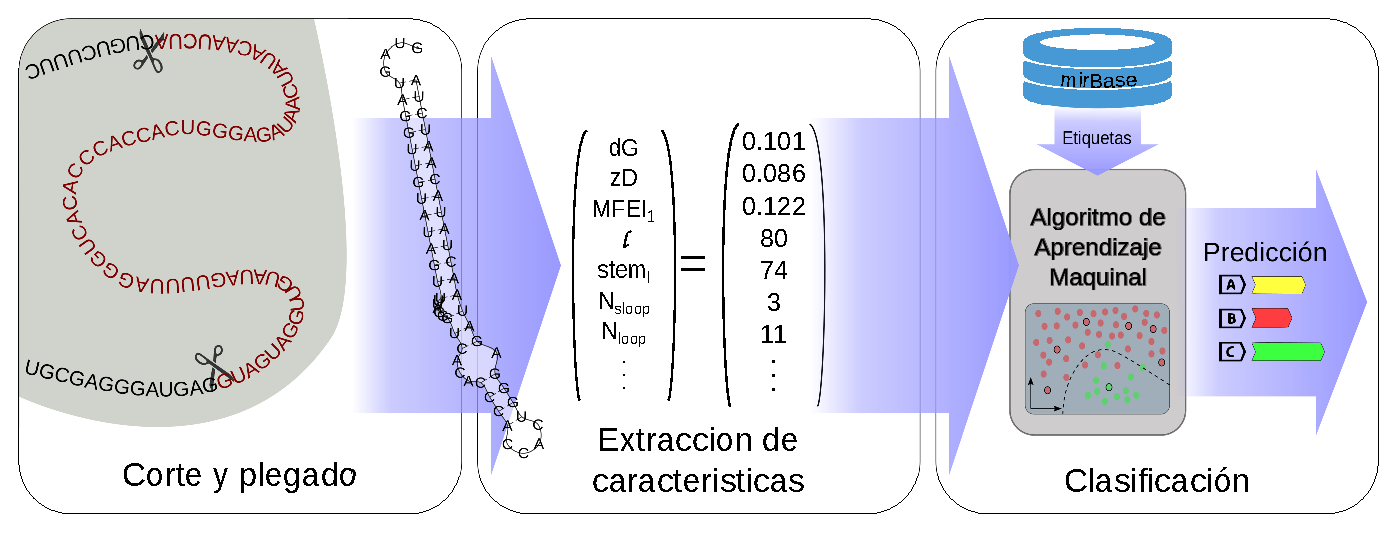
\includegraphics[width=\textwidth]{fig/diagrama.eps}
	\caption[Etapas de la predicción de microARN]{Proceso completo de predicción de nuevos pre-miARNs, separado en sus tres etapas principales.}
	\label{fig:esquema}
\end{figure}

\subsection{Ventaneo del genoma}

Se comienza cortando el genoma completo en ventanas solapadas de una longitud varias veces mayor (500 nt.) a la de un pre-miARN promedio. La ventana debe ser lo
suficientemente larga para poder capturar la horquilla completa pero además para que se tenga en cuenta el entorno de cualquier posible horquilla al estimar la
estructura secundaria. Esto último es muy importante ya que los resultados de estimar la estructura secundaria se ven muy afectados por el entorno de la
secuencia. Por ejemplo, sin considerar el entorno de una secuencia, la estructura secundaria estimada puede presentar una estabilidad menor a la que se formaría
si se habría considerado el entorno.

\subsection{Plegado y poda}

Se predice la estructura secundaria que formaría cada una de las ventanas al plegarse. Para ello se utiliza el algoritmo de mínima energía libre
\citep{zuker1981optimal}. Este algoritmo utiliza programación dinámica para encontrar la estructura secundaria que minimiza la energía liberada. Dado que las
ventanas utilizadas son relativamente largas, las estructuras normalmente presentan múltiples bucles. Por lo tanto, el siguiente paso es buscar los puntos de
corte que logren separar la estructura completa en varias estructuras tipo horquilla, como se puede ver en la Figura~\ref{fig:hextractor}. De las horquillas
extraídas, se eliminan las que no superan una longitud y nivel de emparejamiento mínimo y el resto pasa a la siguiente etapa.

\subsection{Recorte de secuencias}

Como se utilizan ventanas de una longitud varias veces mayor a la de un pre-miARN promedio, generalmente las secuencias encontradas forman estructuras
secundarias mayores a la de un pre-miARN. Por este motivo es importante analizar cada secuencia para detectar si es necesario un recorte. Como aún se desconoce
el funcionamiento de las enzimas que se encargan de separar el pre-miARN de la secuencia, se utilizan ciertas heurísticas que permiten obtener secuencias con
longitudes y estabilidad similares a las de un pre-miARN. Estas reglas optimizan la energía libre mínima normalizada por la longitud de la secuencia (NMFE, por
sus siglas en ingles \textit{Normalized Minimum Free Energy}). Aunque se pueden encontrar puntos de corte óptimos re-estimando la estructura secundaria para
todos los posibles cortes, utilizar reglas heuristicas proporciona más flexibilidad y acelera el proceso. Primero, la secuencia debe exceder una longitud
mínima, predefinida según la especie en estudio. De esta manera, se puede asegurar que la estructura secundaria tenga una longitud suficiente para ser un
pre-miARN de la especie en análisis. En segundo lugar, los cortes se realizan en el primer nucleótido no emparejado de un bucle interno o bulto de la
estructura secundaria (comenzando desde el bucle principal). Para elegir el bucle o bulto donde cortar se asigna una puntuación a cada imperfección como $ S (1
- D / L) ^ 2 $, donde $ S $ es la longitud de la imperfección, $ D $ es la distancia al bucle principal y $ L $ es la longitud del tallo (desde el lazo
principal hasta el último nucleótido emparejado). Si las imperfecciones en la estructura secundaria son grandes, es probable que cortar la secuencia en esos
puntos genere una estructura con menor NMFE. Por otra parte, cuanto menor es la longitud de la secuencia (independientemente del nivel de emparejamiento), mayor
es la NMFE. Por lo tanto, se favorecen los bucles o bultos más cercanos al bucle principal.

\begin{figure}[tpb]
	\centering
	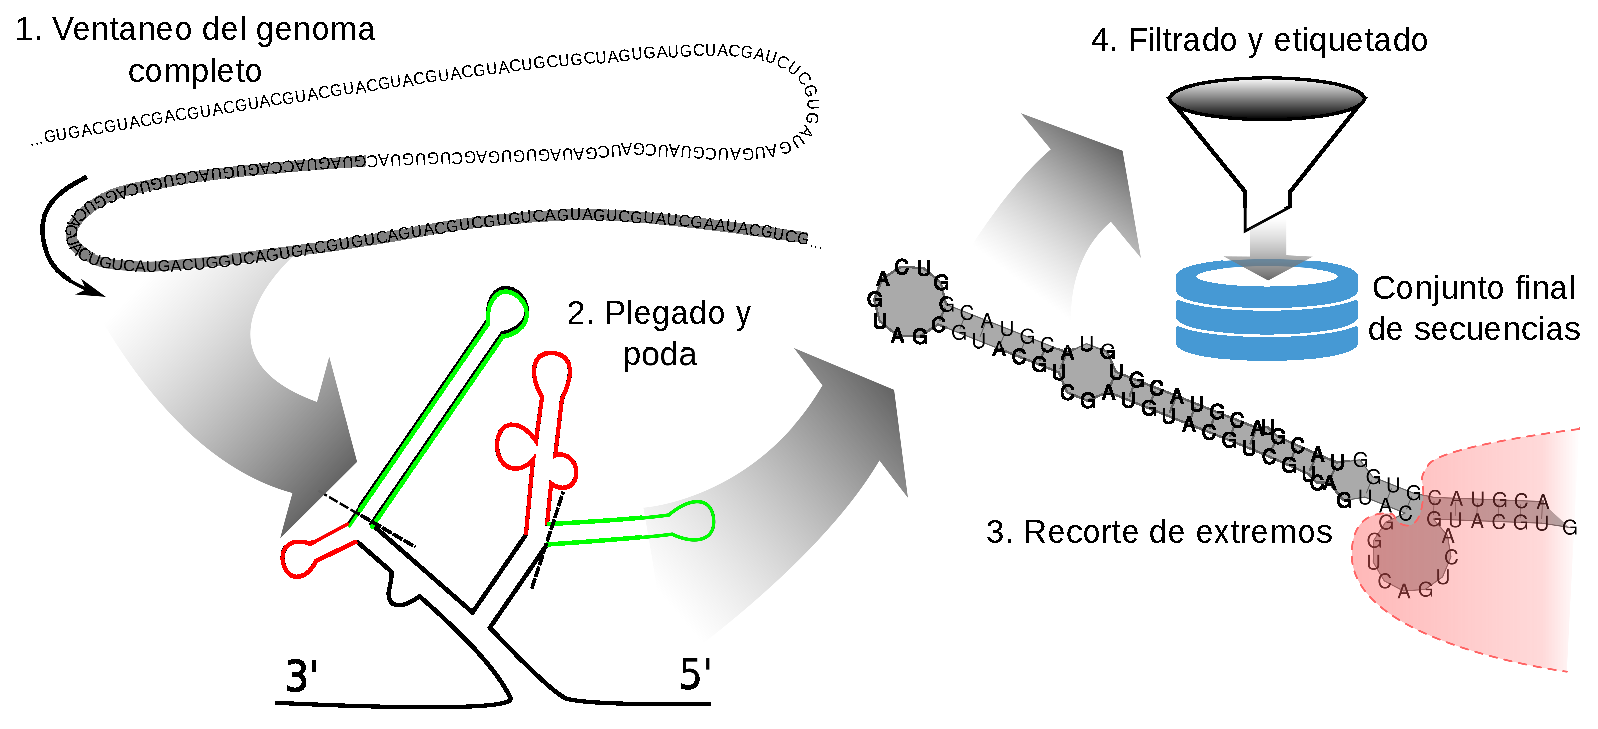
\includegraphics[width=\textwidth]{fig/hextractor.eps}
	\caption[Extracción de secuencias tipo tallo-horquilla]{Proceso de extracción de secuencias tipo tallo-horquilla del genoma completo.}
	\label{fig:hextractor}
\end{figure}


\subsection{Filtrado de repetidas}

Las secuencias repetidas se eliminan para evitar costo computacional extra en las siguientes etapas. Estas secuencias repetidas además perturban los
resultados de los algoritmos de predicción utilizados en la última etapa, ya que cada repetición aumenta la “importancia” que se le da a una secuencia.
 Dado que la ventana se mueve de forma solapada, es posible que una estructura secundaría sea capturada más de una vez. Estas repeticiones aparecen de forma
 consecutiva y son secuencias casi idénticas. Entonces, lo único que puede variar es la longitud, dado que una horquilla puede caer en uno de los extremos de la
 ventana, generando una horquilla más corta. Para eliminarlas se realiza una comparación de cada secuencia con las últimas secuencias extraídas. Si una de las
 secuencias contiene a la otra, la más corta se elimina.

\section{Extracción de características}

La extracción de características de pre-miARN consiste en convertir las secuencias de nucleótidos (representadas como cadenas de caracteres) en vectores
numéricos. De esta manera se pueden aplicar técnicas de aprendizaje maquinal para lograr separar las secuencias pre-miARN de las que no lo son. Como antes se
expresó, se han presentado muchas características que pueden usarse para representar secuencias de ARN \citep{Lopes2014}, pero la variedad de herramientas para
extraerlas son un problema que dificulta su utilización. Estas tienen diferentes interfaces de acceso (web, línea de comandos, interfaz gráfica, etc.) y no
siempre son de libre acceso. Para resolver este problema se creó una biblioteca que implementa de forma unificada todos los procesos de extracción publicados en
la literatura en los últimos 10 años. Esta herramienta puede extraer características de la mayoría de los métodos de predicción de miARN de los últimos años:
Triplet-SVM \citep{xue2005classification}, RNAmicro \citep{hertel2006hairpins}, BayesMiRNAfind \citep{yousef2006combining}, MiRFinder
\citep{huang2007mirfinder}, MiPred \citep{jiang2007mipred}, miRRim \citep{terai2007mirrim}, microPred \citep{batuwita2009micropred}, miRanalyzer
\citep{hackenberg2009miranalyzer}, MiRenSVM \citep{ding2010mirensvm} y miPredGA \citep{xuan2011genetic}.

La biblioteca, llamada miRNAfe, se construyó de forma modular para facilitar el proceso de agregar nuevos algoritmos de extracción de características en el
futuro. Además de la biblioteca, se creó una interfaz web para simplificar el acceso a usuarios del dominio de aplicación sin conocimientos de programación.
Tanto la biblioteca como la versión web pueden calcular hasta 80 características donde muchas son matrices multidimensionales. Las características se han
dividido en seis grupos predefinidos: secuencia primaria, estructura secundaria, estabilidad termodinámica, estabilidad estadística, conservación entre genomas
de diferentes especies y análisis de subcadenas de las secuencias. En las próximas secciones se detalla en qué consiste cada grupo de características. Una lista
completa de las características descritas con mayor detalle se presentan en el Anexo~\ref{sec:mirnafe}.


\subsection{Secuencia primaria}

Estas son las características más simples y representan información de la secuencia principal. MiRNAfe puede extraer un total de 5 características en este
grupo: longitud de la secuencia ($\ell$), proporción de cada base en la secuencia, proporción de dinucleótidos, contenido de guanina y citosina y relación
guanina-citosina. Las dos últimas características se definen como:

\begin{equation} \label{eq:contenidoGC}
	{G+C}_{content} = \frac{G+C}{G+C+A+U},
\end{equation}
\begin{equation} \label{eq:GCratio}
	{GC}_{ratio} = \frac{G}{C},
\end{equation}

\noindent donde $G$, $C$, $A$ y $U$ representan la cantidad de cada base encontrada en la secuencia \citep{hertel2006hairpins}. Todas estas características
forman un vector de 23 elementos, compuesto por: las 4 proporciones base, las 16 proporciones de dinucleótidos, la longitud de la secuencia, ${G+C}_{contenido}$
y ${GC}_{ratio}$. Aunque estas características son bastante simples, han mostrado un alto poder discriminatorio \citep{batuwita2009micropred}, y por lo tanto se
usan en la mayoría de herramientas de predicción.

\subsection{Estructura secundaria}

Estas características representan información de la estructura secundaria y son el grupo más numeroso. La característica más utilizada de este grupo, quizás por
ser una de las primeras publicadas para la predicción de pre-miARN, es la proporción de tripletas \citep{xue2005classification}. Una tripleta es un elemento
formado con el estado de estructura (emparejado o no emparejado) de tres nucleótidos y el tipo de base del nucleótido del medio. Un ejemplo de una tripleta es
``. ((A '', donde el paréntesis representa un nucleótido emparejado, un punto uno no emparejado, y la letra es la base del nucleótido del medio. Como hay 2
estados posibles para un nucleótido y 4 bases diferentes, se pueden formar 32 tripletas ($4\times2^{3} $). El número de ocurrencias de cada elemento en la
secuencia se cuenta y se normaliza para producir un vector de 32 características. Un enfoque similar a las tripletas fue utilizado por
\cite{huang2007mirfinder}, que propuso otra representación para la estructura secundaria. En primer lugar, se definen cinco símbolos para indicar el estado de
cada par de bases en el tallo: `$=$'', ``$:$'', ``$-$'', ``$.$'' y ``$\wedge$''. Cada uno de ellos corresponde al estado de coincidencia, falta de coincidencia,
eliminación, inserción por bucle interior e inserción por bulto, respectivamente. Luego, al tomar dos símbolos adyacentes, se pueden formar 14 posibles
combinaciones, cada una de las cuales tiene un significado especial. Por ejemplo: ``$=-$'', ``$=.$'', y``$=:$'' representan el límite del bucle principal, y
``$:\wedge$'' representa que el bucle es asimétrico. La frecuencia de cada combinación se usa como un vector de características. Esta representación también se
puede usar para calcular cuatro características: $pMatch$, $pMismatch$, $pDI$ y $pBulge$ \citep{huang2007mirfinder}. Estas características se calculan sobre
supuestos miARN maduros, seleccionados como la región de 22 nucleótidos donde el apareamiento de bases es máximo. Representan la frecuencia de
emparejamiento de bases, la frecuencia de no emparejamiento, las frecuencias de borrado e inserción y la simetría de los bucles abombados, respectivamente.

Otro tipo de características se relaciona con estructuras llamadas tallos, que son motivos estructurales que contienen más de tres pares de bases contiguas
\citep{ng2007novo}. Estas características son el número de tallos, la proporción de cada posible par de bases por tallo, el número promedio de pares de bases
por tallo y la longitud del tallo más largo. El resto de las características son la longitud de la región del tallo (es decir, la cantidad de nucleótidos de la
horquilla sin contar los que se encuentran en el bucle principal, que no se debe confundir con los llamados tallos en \cite{ng2007novo}), longitud del bucle
terminal, número de bucles, número de bultos, longitud de bucle más largo, número de bucles simétricos y asimétricos, nucleótidos en bucles simétricos y
asimétricos, región simétrica más larga, longitud promedio de bucles simétricos, longitud promedio de bucles asimétricos, cantidad de bultos y bucles de
longitud $ 1,2, ..., 6$ y mayor que $7$, número de pares de bases, proporción de pares de bases, proporción de pares de bases ajustada y $G+C_{contenido}$ en el
bucle terminal \citep{Lopes2014}. Finalmente, la biblioteca permite calcular el recuento de lecturas a partir de los datos de RNAseq. Esta característica
necesita que el usuario proporcione un archivo adicional con lecturas, que se alinea con las secuencias analizadas y cuenta sus correspondencias.

\subsection{Estabilidad termodinámica}

La característica más utilizada de este grupo es la energía mínima libre ($MFE$, por sus siglas en ingles \textit{Minimum Free Energy}): la energía estimada que
una secuencia libera cuando se pliega en la estructura secundaria más estable \citep{zuker1981optimal}. La energía libre del conjunto ($EFE$) tiene un
significado similar y se obtiene con el algoritmo de \cite{mccaskill1990}. Otras características de este grupo se calculan como combinaciones de esos valores.
Por ejemplo, el índice MFE 1 ($MFEI_{1}$) es la relación entre la energía libre mínima y el ${G+C}_{contenido}$ definido en (\ref{eq:contenidoGC}). Del mismo
modo, se puede calcular la diferencia $MFE-EFE$, $MFE$ ajustado, $MFEI_{2}$, $MFEI_{3}$ y $MFEI_{4}$ \citep{batuwita2009micropred}. También hay algunas
características que utilizan enfoques teóricos de información para estimar la confianza de la estructura secundaria predicha, como la entropía ajustada de
Shannon de las probabilidades de emparejamiento \citep{ng2007novo}, definida como

\begin{equation}
	\label{eq:dQ}
	dQ = \frac{1}{\ell} \sum_{i<j} p_{ij} \log_2 p_{ij} ,
\end{equation}

\noindent donde $p_{ij}$ es la probabilidad de que el nucleótido $i$ forme un par con el nucleótido $j$ y $\ell$ es la longitud de la secuencia. Las
probabilidades de cada par se calculan con el algoritmo de \cite{mccaskill1990}. Otro ejemplo es la distancia de pares ajustada, definida como

\begin{equation}
	\label{eq:dD}
	dD = \frac{1}{\ell} \sum_{i<j} p_{ij} (1 - p_{ij}).
\end{equation}

Además, en este grupo se puede calcular la frecuencia del conjunto, la diversidad, el potencial del tallo 3\textquoteright~ y 5\textquoteright~, y el
potencial del bucle \citep{terai2007mirrim}. Hay 15 funciones en este grupo, que se describen con más detalle en el Anexo~\ref{sec:mirnafe}.

\subsection{Estabilidad estadística}

Se sabe que los precursores que contienen un miARN son más estables que las secuencias aleatorias. Las características de este grupo se calculan como la
puntuación estándar (z-score) de cualquier característica relacionada con la estabilidad \citep{bonnet2004evidence}. Para calcular este valor, se debe generar una
población aleatoria de secuencias intercambiando las bases de la secuencia analizada. De esta forma, las secuencias generadas artificialmente conservan las
proporciones de nucleótidos o incluso la proporción de dinucleótidos si algunos intercambios están restringidos (la herramienta tiene una opción para
elegir qué método de intercambio usar). Utilizando las secuencias generadas, la estabilidad de la secuencia original se puede medir con

\begin{equation}
	z = \frac{x-\mu}{\sigma},
\end{equation}

\noindent donde $x$ es el valor original de alguna característica relacionada con la estabilidad, $\mu$ es la media y $\sigma$ es la desviación estándar de la
población de secuencias generada aleatoriamente. Este puntaje representa, para un valor, cuántas desviaciones estándar un valor está por encima de la media de
la población. Por lo tanto, un puntaje z negativo indica una secuencia que es estadísticamente más estable que la media de la población. Otra estadística
utilizada para medir la estabilidad de la secuencia en comparación con secuencias aleatorias es el valor $p$. Se calcula como la proporción de secuencias
aleatorias que son más estables que la secuencia analizada. Por lo tanto, un bajo valor de $p$ indica que la secuencia analizada es una de las secuencias más
estables generadas con esa proporción de nucleótidos (o dinucleótidos). Las medidas de estabilidad que se pueden normalizar con z-score son:
\begin{itemize}
	\item $ MFE $ ($ zMFE $);
	\item $ EFE $ ($ zEFE $);
	\item $ MFE $ ajustado ($ zG $);
	\item entropía de Shannon ($ zQ $);
	\item propensión de pares de bases ($ zP $) \citep{ng2007novo} y
	\item distancia de pares de bases ($ zD $) \citep{ding2010mirensvm}.
\end{itemize}

El valor $p$ se puede usar para normalizar $ MFE $ ($ pMFE $) \citep{bonnet2004evidence} y $ EFE $ ($ pEFE $) \citep{ding2010mirensvm}. Aunque el z-score y el
$p$-value son similares, a menudo se usan juntas en predicción ya que pueden tomar valores muy diferentes \citep{ding2010mirensvm}. En resumen, se pueden
calcular 8 características en este grupo. Además se puede especificar el método de mezcla (preservación de la composición de nucleótidos o dinucleótidos) y el
número de secuencias aleatorias generadas.

\subsection{Conservación filogenética}

Cuando una parte del genoma se conserva entre especies relacionadas, es muy probable que tenga un papel importante en el genoma. Las características de este
grupo miden el nivel de conservación entre secuencias de especies relacionadas filogenéticamente. Todas las características se calculan sobre alineaciones de
dos o más secuencias que el usuario debe proporcionar. Algunas características no sólo tienen en cuenta el nivel de conservación, sino también la estabilidad
termodinámica. Las características de ese grupo son:
\begin{itemize}
	\item frecuencia de mutación \citep{huang2007mirfinder}, que es la proporción de bases que difieren de una secuencia a otra;
	\item entropía del brazo 5\textquoteright~, el brazo 3\textquoteright~, la región del bucle y la entropía mínima (la menor entropía de las
		calculadas sobre una región de 21 nucleótidos \citep{hertel2006hairpins});
	\item número de diferencias en la estructura secundaria dividido por el número de diferencias entre las secuencias \citep{huang2007mirfinder};
	\item promedio de $MFE$, $dG$ y $MFEI_{1}$;
	\item diferencia de $MFE$ entre dos secuencias alineadas dividida por el número de diferencias entre las secuencias \citep{huang2007mirfinder};
	\item energía libre de la estructura secundaria de consenso;
	\item conservación del brazo 3\textquoteright~ y del brazo 5\textquoteright~ y
	\item puntaje de conservación \citep{terai2007mirrim}, que se calcula usando dos procesos de Markov, uno que se mueve en la dimensión de tiempo (sobre
		las ramas del árbol de evolución) y el otro en dimensión espacial (sobre la secuencia);
\end{itemize}

Se pueden extraer un total de 14 características en este grupo, que se describen en detalle en el Anexo~\ref{sec:mirnafe}.

\subsection{Análisis de subcadenas de 22 nt}

Estas características se calculan en todas las subcadenas de 22 nt dentro de una secuencia determinada. Se basan en el hecho de que si una secuencia es un
pre-miARN, una de las subcadenas analizadas tiene que ser el miARN maduro y las características calculadas deben capturar sus particularidades. Como
resultado, se obtiene una matriz con longitud $ n = \ell - 22 $, donde el elemento $i$-th representa el valor de la característica calculada sobre la
subcadena que comienza en la base $i$. MiRNAfe puede extraer las siguientes 5 características en este grupo:
\begin{itemize}
	\item probabilidad de emparejamiento de bases en la subcadena \citep{lim2003}, que es la suma de probabilidades de emparejamiento de bases sobre la subcadena;
	\item suma de bases no emparejadas en la subcadena;
	\item suma de probabilidades de emparejamiento de bases en la estructura secundaria sin las probabilidades de los nucleótidos de la subcadena;
	\item simetría de bultos, como la diferencia entre la cantidad de bases no emparejadas en cada brazo de la subcadena;
	\item distancia desde la subcadena hasta el bucle terminal.
\end{itemize}

\section{Clasificación de pre-miARNs}

En esta etapa se utilizan pre-miARNs conocidos del genoma de la especie de interés para entrenar un clasificador que realizará predicciones sobre otras
secuencias de ARN, sobre las cuales no se  conoce su función. Las secuencias de pre-miARN utilizadas como ejemplos para el entrenamiento pueden ser tomadas de
alguna base de datos de pre-miARNs como  mirBase \citep{kozomara2014mirbase}, mientras que las secuencias no etiquetadas son el resultado del corte y plegado
del genoma crudo. Como antes se mencionó, utilizar métodos de aprendizaje maquinal supervisado presenta numerosas limitaciones. Como enfoque más novedoso y
superador del problema, se desarrolló un clasificador semi-supervisado que aprenda la distribución de secuencias del genoma analizado en el espacio de las
características, utilizando las secuencias no etiquetadas. Aprovechando la información que aportan estas secuencias, se pretende mejorar las tasas de predicción
en situaciones donde la cantidad de ejemplos es baja o cuando no son representativos de sus respectivas clases.

Durante la última década, una de las áreas más activas en el aprendizaje semi-supervisado ha sido la de los métodos basados en grafos, donde cada nodo
representa un punto de datos, y un borde conecta nodos si son de alguna manera similares. Luego, utilizando los nodos etiquetados, se obtienen etiquetas
pronosticadas para el resto de los nodos sin etiqueta. Estos métodos han mostrado buenas tasas de predicción \citep{joachims2003transductive} y han podido
manejar grandes volúmenes de datos. Se ha desarrollado un nuevo algoritmo de predicción de este tipo que tiene en cuenta las características particulares del
problema: a) grandes volúmenes de datos; b) desbalance de clases muy alto; c) clase negativa mal representada o directamente ausencia de ejemplos negativos. A
continuación se describe el nuevo clasificador propuesto, denominado miRNAss.

%****************************************************************************************
\begin{figure}[tpb]
	\centering
	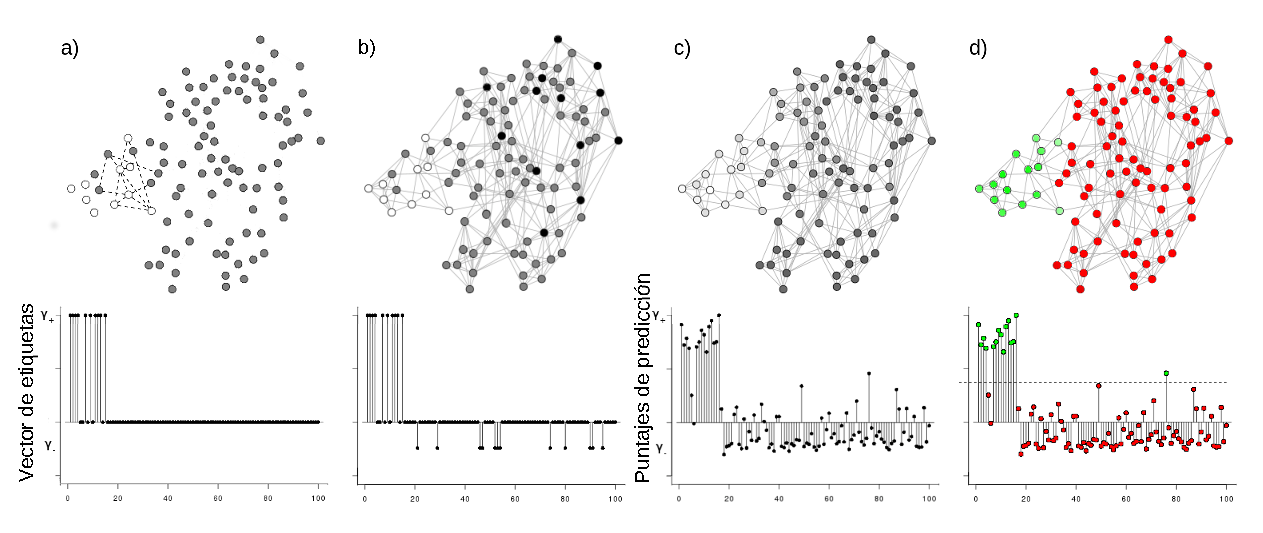
\includegraphics[width=\linewidth]{fig/workflow.eps}
	\caption[Evolución del grafo]{Evolución simplificada del grafo, el vector de etiquetas y el vector de puntajes de predicción en los 4 pasos del método
	propuesto: a) Construcción de grafo; b) inicialización de conjunto negativo; c) Estimación de puntajes de predicción; d) optimización del umbral.}
	\label{fig:workflow}
\end{figure}
%****************************************************************************************

MiRNAss recibe como entrada un conjunto de vectores de características $m$-dimensional $\mathbf{x}_{i}$, que representan secuencias, y un vector
correspondiente de etiquetas $\Bell$. El elemento $i$-th en el vector de etiquetas tiene un valor positivo $\gamma_{+}$ si la secuencia $i$-th es un pre-miARN
conocido, un valor negativo $\gamma_{-}$ si no es un pre-miARN, y cero si es una secuencia desconocida que debe ser clasificada por el método. El método
tiene cuatro pasos: 1) construcción de un grafo donde cada nodo representa una secuencia; 2) busqueda de ejemplos negativos, si no se proporcionan; 3) estimación
de los puntajes de predicción para cada nodo en el grafo; y 4) estimación de un umbral óptimo para separar las secuencias en dos clases.

La Figura~\ref{fig:workflow} muestra un ejemplo de la aplicación del método. En este ejemplo, 15 secuencias son verdaderos pre-miARN y el resto son secuencias
no pre-miARN. En la Figura~\ref{fig:workflow}.a, el grafo se construye y se asignan los valores iniciales a $\Bell$: valores positivos ($\gamma_{+}$) a los
ejemplos conocidos de pre-miARNs. En la Figura~\ref{fig:workflow}.b, algunos nodos que están topológicamente lejos de los ejemplos positivos se etiquetan como
ejemplos negativos ($\gamma_{-}$). Los nodos del grafo están coloreados de acuerdo con los valores en el vector $\Bell$. En la Figura~\ref{fig:workflow}.c,
los puntajes de predicción se estiman para todas las secuencias, teniendo en cuenta que: i) tienen que ser suaves; es decir, las secuencias topológicamente
cercanas en el grafo deben tener puntajes de predicción similares; y ii) los puntajes tienen que ser similares a los valores distintos de cero dados en el
vector de etiqueta $\Bell$. Finalmente, usando los puntajes de predicción asignados a los ejemplos marcados se estima un umbral óptimo para separar los
pre-miARN de las otras secuencias. Las secuencias que pasan el umbral están coloreadas en verde; el resto, en rojo.

\subsection{Construcción del grafo}

Al construir el grafo, cada nodo representa una secuencia y cada arista une dos nodos si las secuencias son similares en el espacio de las características. Para
medir la similaridad se utiliza la distancia euclidea entre los vectores de características. Si una característica no ayuda realmente a discriminar entre
clases, puede empeorar el rendimiento del clasificador. Por lo tanto, es importante preprocesar los vectores de características para ponderar adecuadamente cada
característica de acuerdo con su poder de predicción. Un algoritmo que ha demostrado mejorar los resultados en clasificadores que son sensibles a la función de
distancia es el algoritmo RELIEF-F \citep{kononenko1994estimating, wettschereck1997review}. Además, es computacionalmente eficiente y puede usarse para grandes
volúmenes de datos. Funciona de la siguiente manera: comenzando con un vector de pesos con $m$ ceros, para cada ejemplo busca el ejemplo más cercano de la misma
clase y el ejemplo más cercano que pertenezca a la otra clase. Luego, aumenta los pesos de las características que son similares al ejemplo de la misma clase y
diferentes al ejemplo de la otra clase. Por el contrario, se reducen los pesos de las características que son diferentes al ejemplo de la misma clase o
similares al ejemplo de la otra clase. El resultado se llama vector de relevancia y tiene valores altos para las características más discriminativas. Si la
relevancia de una característica es negativa, entonces no ayuda a discriminar entre clases y por lo tanto puede ser eliminada. El resto de las características se escala
por su puntaje de relevancia para dar más peso a las más discriminativas.

Para la construcción del grafo, una opción común es el algoritmo de $k$-vecinos más cercanos (KNN), dado que es simple, rápido, eficiente en uso de
memoria y fácilmente paralelizable. KNN construye una matriz de adyacencia ponderada por similitud con elementos

\begin{equation}
	a_{ij} =
	\begin{cases}
		\frac{\mu}{\mu + ||\mathbf{x}_{i} - \mathbf{x}_{j}||^2} & \text{si} \ \mathbf{x}_{j} \in  \mathcal{K}(\mathbf{x}_{i}) \ \text{y} \ \ell_{i}
		\ell_{j} \geq 0 \\
		0 & \text{en otro caso,} \\
	\end{cases}
\end{equation}

\noindent donde $\mathbf{x}_{i}$ es el vector de características correspondiente a la secuencia $i$-th, $\mathcal{K} (\mathbf{x}_{i})$ es el conjunto de los
$k$ vecinos más cercanos de $\mathbf{x}_{i}$, y $\mu$ es la media de las distancias entre las secuencias conectadas y se  utiliza para normalizar los pesos de
las aristas.

\subsection{Búsqueda de ejemplos negativos}

\floatname{algorithm}{Algoritmo}
\renewcommand{\algorithmicrequire}{\textbf{Entrada:}}
\renewcommand{\algorithmicensure}{\textbf{Salida:}}
\renewcommand{\algorithmicrepeat}{\textbf{repetir}}
\renewcommand{\algorithmicuntil}{\textbf{mientras}}
\renewcommand{\algorithmicreturn}{\textbf{delvolver}}
\begin{algorithm}[tpb]
	\caption{Búsqueda automática de ejemplos negativos}
	\label{algNS}
	\begin{algorithmic}[1]
		\REQUIRE{matriz de adyacencia $A$, vector de etiquetas $\Bell$ con ceros y valores positivos únicamente, número de ejemplos negativos a etiquetar $T$.}
		\ENSURE{vector $\Bell$ con $T$ etiquetas negativas asignadas.}
		\STATE{$s_{i} = \begin{cases}
				1 & \text{si} \quad \ell_{i} > 0 \\
				0 & \text{en otro caso} \\
		\end{cases}$}
		\REPEAT
		\STATE{$s_{i} = \max_{\forall j \neq i}\limits \, \{s_{i}, a_{ij} s_{j} \}, \quad \forall i$}
		\UNTIL{no hay cambios en $\mathbf{s}$}
		\STATE{$p_i=e^{1-s_i}-1,\quad \forall i$}
		\STATE{Muestrear $T$ elementos de $\Bell$ usando $\mathbf{p}$ como pesos para la selección}
		\STATE{Etiquetar elementos elegidos como clase negativa}
		\RETURN $\Bell$
	\end{algorithmic}
\end{algorithm}

Si sólo se cuenta con ejemplos positivos, la matriz de adyacencia se puede utilizar para etiquetar un conjunto de secuencias como ejemplos negativos. La idea
clave es seleccionar aleatoriamente algunas secuencias sin etiqueta entre las más distantes a los ejemplos positivos. De esta forma, la probabilidad de
etiquetar incorrectamente un pre-miARN bien conocido como un ejemplo negativo será baja. Para ello, se calcula una medida de la similitud de cada secuencia con
los ejemplos positivos utilizando la distancia topológica. Este vector de similitud, llamado $\mathbf{s}$, se inicializa con $+1$ en los elementos
correspondientes a ejemplos positivos. Los nodos sin etiqueta se inicializan con $0$. Entonces, se puede usar un método iterativo para actualizar las
similitudes en $\mathbf{s}$ (ver Algoritmo~\ref{algNS}). En cada iteración y para cada nodo, el valor de similitud correspondiente de cada vecino se multiplica
por los pesos de aristas correspondientes que los conectan. El valor máximo de los resultados obtenidos para cada vecino se compara luego con el valor de
similitud actual del nodo. Si es más alto, se actualiza el valor de similitud del nodo. Cuando no hay más cambios en $\mathbf{s}$, se seleccionan $T$ secuencias
de forma aleatoria usando como probabilidad de selección $p_{i} = e^{1 - s_{i}} -1$ y se etiquetan como ejemplos negativos.

\subsection{Estimación de puntajes de predicción}

En el tercer paso, los puntajes de predicción se calculan resolviendo un problema de optimización \citep{joachims2003transductive}. Como se dijo anteriormente,
se deben considerar dos puntos: i) los puntajes de predicción deben ser topológicamente suaves; y ii) las predicciones deben ser similares a las etiquetas
conocidas. Para suavizar la predicción se minimiza el cuadrado de las diferencias entre las puntuaciones de predicción de las secuencias adyacentes. Una
representación conveniente para calcular fácilmente estas diferencias es el laplaciano normalizado del grafo \citep{shi2000normalized}, definido
como

\begin{equation*}
	L=I-D^{-1/2}AD^{-1/2}
\end{equation*}

\noindent donde

\begin{equation*}
	D_{ij} =
	\begin{cases}
		\sum_{k=0}^n A_{ik} & \text{si } i=j \\
		0 & \text{en otro caso.} \\
	\end{cases}
\end{equation*}

\noindent El Laplaciano tiene una propiedad útil para medir la suavidad de la solución. Supongamos $\mathbf{z} \in \mathbb{R} ^ N$, con una predicción para cada nodo
del gráfico. Entonces,

\begin{equation}
	\begin{split}
		\mathbf{z}^T L \mathbf{z} & = \mathbf{z}^T I \mathbf{z} - \mathbf{z}^T {D^{-1/2}}^T A D^{-1/2} \mathbf{z} = \\
					  & = \sum_{i}^{n} z_{i}^{2} -  \sum_{i}^{n}  \sum_{j}^{n} \frac{z_{i}}{\sqrt{d_{ii}}} \frac{z_{j}}{\sqrt{d_{jj}}}
		a_{ij} = \\
		& = \frac{1}{2} \sum_{i}^{n} \sum_{j}^{n} a_{ij} \left(\frac{z_{i}}{ \sqrt{d_{ii}}} - \frac{z_{j}}{\sqrt{d_{jj}}}
	\right)^{2}.
\end{split}
\end{equation}

\noindent Esta última expresión muestra que $\mathbf {z} ^ T L \mathbf {z}$ mide la diferencia al cuadrado entre las predicciones $z_{i}$ y $z_{j}$, ponderados
por $a_{ij} $. Si las secuencias $ i $ y $ j $ son similares, y por lo tanto $ a_{ij} $ tiene un valor relativamente alto, cualquier diferencia entre las dos
predicciones tendrá un alto costo. Si no hay arista que conecte las dos secuencias, $a_{ij} = 0 $ la diferencia entre las predicciones se ignora. Además, se
debe tener en cuenta que las predicciones se ponderan por el inverso de la raíz cuadrada del grado del nodo. Como resultado, los nodos con un grado pequeño se
consideran tan importantes como los nodos altamente conectados.

Entonces, la función objetivo tiene dos componentes: el primer término mide la falta de suavidad de la solución usando la matriz laplaciana normalizada
(componente no supervisada del aprendizaje), y el segundo término es la diferencia al cuadrado entre predicciones y etiquetas distintas de cero en $\Bell$
(componente supervisada). Para aprovechar al máximo el aprendizaje semi-supervisado, no debe haber una gran superposición entre las clases que se separarán. Sin
embargo, si este requisito previo no se cumple, el primer término de la función objetivo no tendrá ningún mínimo importante. Por lo tanto, el segundo término de
la ecuación (el supervisado) conducirá la búsqueda. De esta forma, si no hay una separación clara entre las clases, el método se comportará de forma similar a
cualquier otro método supervisado en las mismas condiciones.

El problema de optimización completo queda definido como

\begin{equation}
	\begin{split}
		\arg\min_{\mathbf{z}} & \qquad \mathbf{z}^TL\mathbf{z} +c(\mathbf{z}-\Bell)^TC(\mathbf{z}-\Bell) \\
		s.t. & \qquad \mathbf{z}^T\mathbf{1} = 0, \\
		     & \qquad \mathbf{z}^T\mathbf{z} = n
	\end{split}
\end{equation}

\noindent donde la combinación de ambas restricciones evita soluciones triviales. En la primera restricción se requiere que la suma de los elementos de
$\mathbf{z}$ sea cero; es decir, las etiquetas de predicción deben tener tanto valores negativos como positivos. La segunda restricción elimina las versiones
escaladas de la solución que, para nuestro propósito, son todas equivalentes.

Los valores $\ell_{i}$ se establecen en $\gamma_{+}$, $\gamma_{-}$ o cero, dependiendo de si la secuencia $ i $-th es positiva, negativa o desconocida,
respectivamente. Como la función objetivo obliga a los valores de $\mathbf{z}$ a acercarse a $\gamma_{+}$ o $\gamma_{-}$, estas constantes deben definirse de
manera tal que la solución óptima $\mathbf{z}^\star$ pueda satisfacer ambas restricciones del problema. Si $n_{+}$ y $n_{-}$ son las cantidades reales de nodos
positivos y negativos en la solución, definiendo $\gamma_{+} = \sqrt{n_{-}/n_{+}}$ y $\gamma_{-}=-\sqrt{n_{+}/n_{-}}$ se consigue que $\mathbf{z}^\star$
satisfaga ambas restricciones. Esto se puede observar al reemplazar $\mathbf{z}^\star$ en las restricciones y asumiendo que este vector tiene $n_{+}$ elementos
iguales a $\gamma_{+}$ y $n_{-}$ iguales a $\gamma_{-}$. Los números $n_{+}$ y $n_{-}$ son generalmente desconocidos, pero se pueden estimar fácilmente a partir
de los ejemplos disponibles. Si se proporcionan ejemplos positivos y negativos para el entrenamiento, se calculará $n_{+}/n_{-}$ como la proporción de ejemplos
dados. Si sólo hay ejemplos positivos, $n_{+}$ se estima como el doble del número de secuencias de entrenamiento y $n_{-} = n - n_{+}$. Esta estimación podría
mejorarse utilizando el conocimiento del dominio, es decir, utilizando el número esperado de miARNs para una especie determinada; sin embargo, no es necesario
ya que el método propuesto no es sensible a estos parámetros (ver Figura~S1 en el Material Suplementario del Anexo~\ref{sec:mirnass}). Por lo tanto, cualquier
valor entre el número de secuencias de entrenamiento positivas y cuatro veces este número se puede utilizar sin impacto en el rendimiento.

La constante $ c $ en la función objetivo se puede usar para establecer el peso relativo del segundo término en comparación con el primero. Un valor grande de
$c$ otorga una mayor penalización a las clasificaciones erróneas, lo que lleva los puntajes de predicción a valores similares a las etiquetas distintas de cero
$ \Bell $. Por el contrario, si se usa un valor bajo de $ c $, las clasificaciones erróneas se penalizan menos y el primer término domina la función objetivo,
lo que produce una solución más suave. La matriz $C$ en el segundo término es una matriz diagonal que tiene valor cero en los elementos correspondientes a
secuencias desconocidas. De esta manera, las secuencias sin etiqueta se ignoran en este término. En los elementos distintos de cero (correspondientes a los
ejemplos etiquetados), el valor asignado permite diferentes penalizaciones por clasificación errónea para cada secuencia. Esta ponderación puede usarse, por
ejemplo, para asignar valores inferiores a los pre-miARN que no han sido validados experimentalmente o que son ejemplos negativos poco confiables. También se
puede usar para evitar la clasificación errónea de ejemplos etiquetados. En la Sección S2 del Material Suplementario del Anexo~\ref{sec:mirnass} se demuestra
que si $ C_ {ii}> (n n _ {+}) / (c n _ {-}) $, la clasificación incorrecta de la secuencia iesima tendrá una mayor penalización que cualquier penalización en
el término no supervisado. Entonces, no puede ser mal clasificado. Como valor predeterminado los elementos distintos de cero de $ C $ se establecen en $ 1 $,
tanto para los ejemplos positivos como negativos.

Para resolver este problema de optimización primero calculamos la descomposición espectral del Laplaciano $ L = U \Sigma U ^ T $. A continuación, utilizamos un
nuevo vector de parámetro $ \mathbf {w} $ tal que $ \mathbf {z} = U \mathbf {w} $. Como el vector propio correspondiente al valor propio más bajo siempre es
constante, la primera restricción del problema de optimización se convierte en $ w_ {1} = 0 $. Si definimos $ V $ como la matriz con todos los vectores propios,
excepto el primero, y $ H $ como la matriz diagonal con todos los valores propios, excepto el más bajo, obtenemos el siguiente problema de optimización

\begin{equation}
	\begin{split}
		\arg\min_{\mathbf{w}} & \quad \mathbf{w}^T H \mathbf{w} + c (V \mathbf{w} - \Bell)^T C (V \mathbf{w} - \Bell) \\
		s.t. & \quad \mathbf{w}^T \mathbf{w} = n.
	\end{split}
\end{equation}

\noindent Definiendo $ Q = H + c V ^ T C V $ y $ b = c V ^ T C \Bell $, este problema puede reescribirse como

\begin{equation}
	\begin{split}
		\arg\min_{\mathbf{w}} &\quad \mathbf{w}^T Q \mathbf{w} + 2 b^T \mathbf{w} + c \Bell^T C \Bell \\
		s.t. &\quad \mathbf{w}^T \mathbf{w} = n,
	\end{split}
\end{equation}

\noindent donde el último término se puede descartar dado que es constante. Usando los multiplicadores de Lagrange el mínimo global de esta función se produce
en $\mathbf {w}^\star = (Q - \lambda^\star I)^{- 1} \mathbf{b} $. Ahora, usando los resultados de \cite{gander1989contrained}, $ \lambda^\star$ se puede
calcular como el menor autovalor de

\begin{equation}
	M = \left( \begin{array}{cc}
			Q & -I \\
	\frac{{\mathbf{b} \mathbf{b}^T}}{{n}} & Q \end{array} \right).
\end{equation}

\noindent A partir de esta solución, las etiquetas se calculan como $ \mathbf {z} ^ \star = V \mathbf {w} ^ \star $.

\subsection{Umbralización de los puntajes de predicción}

Dados los altos desbalances que están presentes en los datos de un genoma completo, es necesario aumentar el costo de clasificación errónea de la clase
positiva. Mientras que la matriz $C$ se puede usar para asignar diferentes costos de clasificación errónea en el proceso de optimización, estimar el umbral que
se aplicará en $\mathbf{z}$ es un método más flexible ya que permite optimizar una única vez y luego elegir la medida de rendimiento a maximizar. Dado que se
espera que los puntajes de predicción ordenen las secuencias de acuerdo a la probabilidad de ser pre-miARNs, modificar el umbral utilizado para separar las dos
clases equivale a clasificar con distintas ponderaciones por clase \citep{mease2007boosted}.

Una métrica de evaluación común que se usa en problemas con desbalance de clases es la media geométrica ($ \bar {G} $) de la sensibilidad y la especificidad $
\bar {G} = \sqrt {S ^ {+} S ^ {-} } $ \citep{batuwita2009micropred, gudys2013huntmi}, donde $ S ^ {+} $ es la proporción de secuencias positivas correctamente
clasificadas como positivas (sensibilidad), y $ S ^ {-} $ es la proporción de secuencias negativas correctamente clasificadas como negativas (especificidad).
Esta medida tiene la ventaja de dar la misma importancia a las clases negativas y positivas, independientemente de la cantidad de elementos en cada clase. Una
mejor medida es el \mbox{F-score}, $ F_ {1} = 2 \, P \, S ^ {+} / (P + S ^ {+}) $, donde $ P $ es la precisión (la proporción de verdaderos positivos dentro de
las secuencias clasificadas como positivas). Cuando se utiliza $ F_ {1} $ para la optimización del umbral se obtiene una mejor $ P $ a costa de una $ S ^ {+} $
más baja. Debido al gran desbalance de clases en este problema de clasificación, es importante prestar especial atención a la cantidad de falsos positivos. Por
lo tanto, $F_{1}$ es una mejor medida para este problema.

Los puntajes de predicción obtenidos para los ejemplos etiquetados se pueden usar para encontrar el umbral que maximice cierta medida de rendimiento objetivo.
Debe señalarse que esto es sólo una estimación, ya que se desconoce la clase real a la que pertenecen las secuencias no etiquetadas. Por esta razón, si
ordenamos los puntajes de predicción $ \mathbf {z} ^ \star $ y calculamos la medida de desempeño utilizando como umbral cada valor de este vector,  entre dos
ejemplos etiquetados consecutivos aparecerán regiones donde esta medida se hace constante. Si el número de ejemplos etiquetados es bajo, estas regiones
constantes pueden ser relativamente grandes. Por lo tanto, el umbral final se establece como el punto medio entre el puntaje de predicción más alto y más
bajo  donde se maximice la medida de rendimiento (ver Figura S3 del anexo~\ref{sec:mirnass}).
